\let\negmedspace\undefined
\let\negthickspace\undefined
\documentclass[journal]{IEEEtran}
\usepackage[a5paper, margin=10mm, onecolumn]{geometry}
%\usepackage{lmodern} % Ensure lmodern is loaded for pdflatex
\usepackage{tfrupee} % Include tfrupee package

\setlength{\headheight}{1cm} % Set the height of the header box
\setlength{\headsep}{0mm}     % Set the distance between the header box and the top of the text

\usepackage{gvv-book}
\usepackage{gvv}
\usepackage{cite}
\usepackage{amsmath,amssymb,amsfonts,amsthm}
\usepackage{algorithmic}
\usepackage{graphicx}
\usepackage{textcomp}
\usepackage{xcolor}
\usepackage{txfonts}
\usepackage{listings}
\usepackage{enumitem}
\usepackage{mathtools}
\usepackage{gensymb}
\usepackage[breaklinks=true]{hyperref}
\usepackage{tkz-euclide} 
\usepackage{listings}
% \usepackage{gvv}                                        
\def\inputGnumericTable{}                                 
\usepackage[latin1]{inputenc}                                
\usepackage{color}                                            
\usepackage{array}                                            
\usepackage{longtable}                                       
\usepackage{calc}                                             
\usepackage{multirow}                                         
\usepackage{hhline}                                           
\usepackage{ifthen}                                           
\usepackage{lscape}
\usepackage{circuitikz}
\usepackage{comment}
\tikzstyle{block} = [rectangle, draw, fill=blue!20, 
    text width=4em, text centered, rounded corners, minimum height=3em]
\tikzstyle{sum} = [draw, fill=blue!10, circle, minimum size=1cm, node distance=1.5cm]
\tikzstyle{input} = [coordinate]
\tikzstyle{output} = [coordinate]


\begin{document}

\bibliographystyle{IEEEtran}
\vspace{3cm}

\title{12.560}
\author{EE25BTECH11026-Harsha}
 \maketitle
% \newpage
% \bigskip
{\let\newpage\relax\maketitle}

\renewcommand{\thefigure}{\theenumi}
\renewcommand{\thetable}{\theenumi}
\setlength{\intextsep}{10pt} % Space between text and floats


\numberwithin{equation}{enumi}
\numberwithin{figure}{enumi}
\renewcommand{\thetable}{\theenumi}

\textbf{Question}:\\
A scalar function is given by $f\brak{x,y}=x^2+y^2$. Take $\hat{i}$ and $\hat{j}$ as the unit vectors along the x and y axes, respectively. At $\brak{x,y}=\brak{3,4}$, the direction along which $f$ increases the fastest is
\begin{enumerate}
\begin{multicols}{4}
    \item $\frac{1}{5}\brak{4\hat{i}-3\hat{j}}$
    \item $\frac{1}{5}\brak{3\hat{i}-4\hat{j}}$
    \item $\frac{1}{5}\brak{3\hat{i}+4\hat{j}}$
    \item $\frac{1}{5}\brak{4\hat{i}+3\hat{j}}$
\end{multicols}
\end{enumerate}
\solution \\
Let us solve the given question theoretically and then verify the solution computationally.\\
\\
\textbf{Approach-1:}
The direction vector along which the function $f\brak{x,y}$ is given by the gradient direction vector of the function, which is given by
\begin{align}
    \nabla f\brak{x,y}=\myvec{\tfrac{\partial f}{\partial x}\\\tfrac{\partial f}{\partial y}}
\end{align}
\begin{align}
    \therefore \nabla f\brak{x,y}=\myvec{2x\\2y}
\end{align}
At $\brak{x,y}=\brak{3,4}$,
\begin{align}
    \nabla f\brak{3,4}=\myvec{6\\8}
\end{align}
\begin{align}
    \implies \text{Direction vector: }\frac{1}{5}\myvec{3\\4}
\end{align}
\newpage
\vspace*{0.25cm}
\begin{figure}[H]
    \centering
    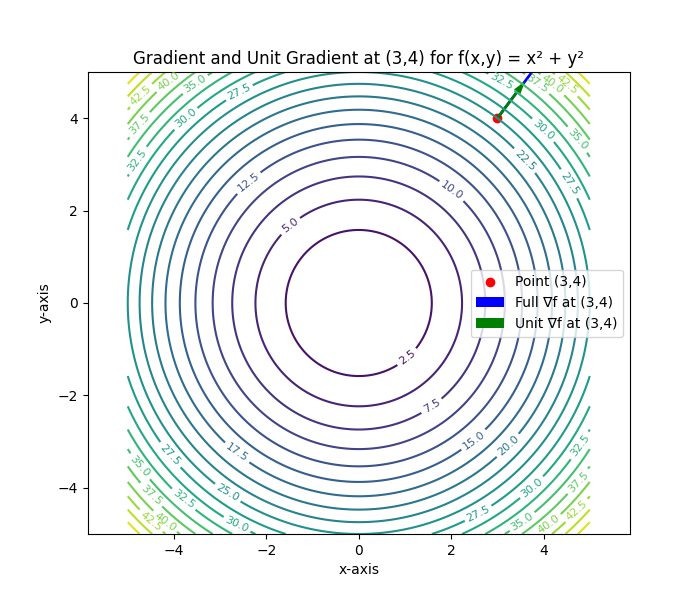
\includegraphics[width=0.7\columnwidth]{figs/Figure_1.png}
    \caption{Graph for approach-1}
    \label{fig:1}
\end{figure}
\textbf{Approach-2: }As the point is given to be $\myvec{3\\4}$, it can be assumed that for the circle,
\begin{align}
    \vec{x}^{\top}\vec{V}\vec{x}=3^2+4^2=25 \label{eq:1}
\end{align}
where $\vec{V}=\vec{I}$.\\
We can infer that the function will increse along the direction vector of normal at that point.
The direction vector of normal is given by
\begin{align}
    \vec{n}=\brak{\vec{V}\vec{q}+\vec{u}}
\end{align}
where, $\vec{q}$ is the point of contact.
\begin{align}
    \therefore \vec{n}=\myvec{1&&0\\0&&1}\myvec{3\\4}+\myvec{0\\0}=\myvec{3\\4}
\end{align}

\newpage
\vspace*{0.25cm}

\begin{figure}[H]
    \centering
    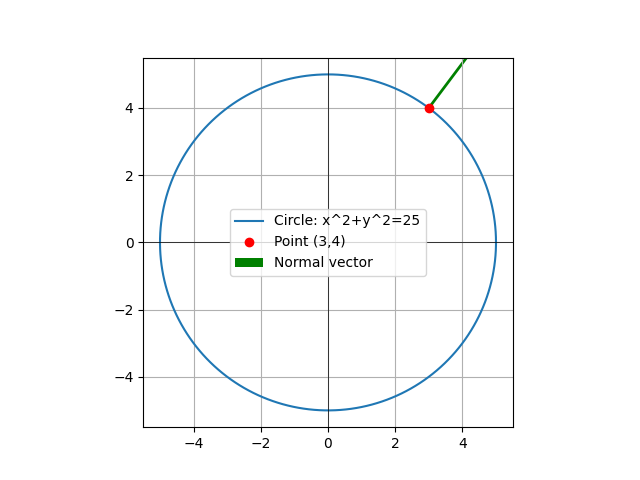
\includegraphics[width=0.7\columnwidth]{figs/Figure_2.png}
    \caption{Graph for approach-2}
    \label{fig:2}
\end{figure}

\end{document}

